\subsection{Composable Tool Architectures (Karsai, Sztipanovits)}

\subsubsection{ Advanced Open Tool Integration Framework (Karsai, Sztipanovits)}

\emph{Formal Specification of Behavioral Semantics} 

ESMoL's time-triggered run-time execution behavior can be realized in a number of ways: via TrueTime, FRODO, or otherwise as long as the tenets of time-triggered behavior are not violated\cite{rt_thesis,gh_truetime}.  During nominal operation, a simplistic time-triggered virtual machine can be modeled as operating in only four states: idle waiting for the next task, initiating the execution of a task, waiting for a task to complete, and a reset at the end of each hyperperiod.  This is illustrated in Fig. \ref{fig:generic_TA}, where the initialization state is collapsed into the execution state.  Each state transition is driven by the execution schedule and therefore by the node's local clock.  In this sense, the VM naturally acts as a timed automaton.  Additional complexity is added by clock synchronization and message passing, but these too can be modeled using concepts present in common timed automata formalisms.

\begin{figure}[thpb]
\centering
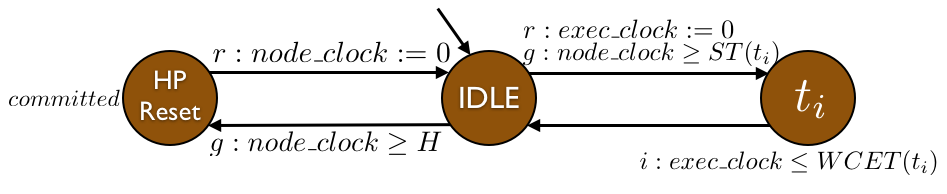
\includegraphics[width=0.75\textwidth]{img/generic_TA.png}
\caption{Basic timed automaton for a single task.}
\label{fig:generic_TA}
\end{figure}

\begin{figure}[thpb]
\centering
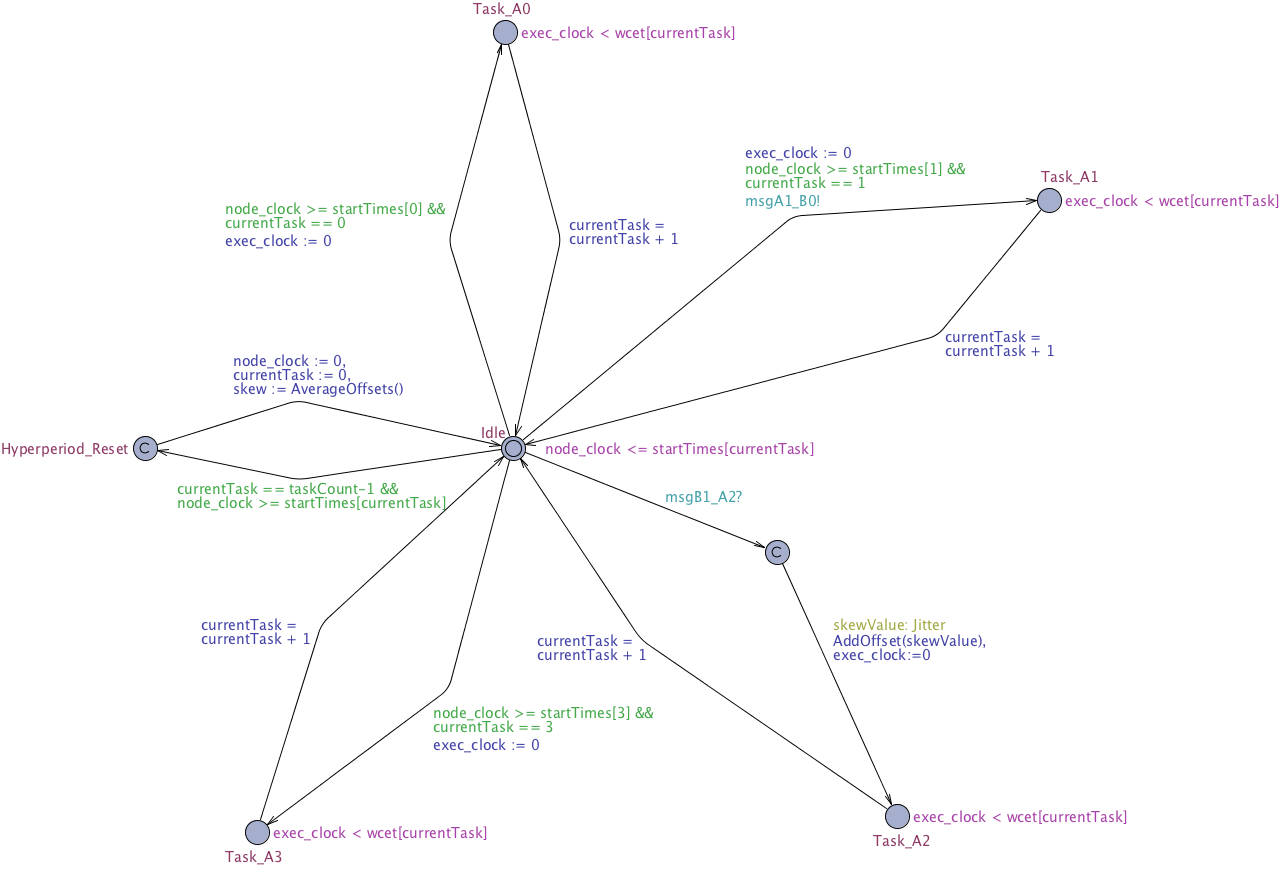
\includegraphics[width=0.75\textwidth]{img/uppaal_nodeA.png}
\caption{UPPAAL model of the task execution on a single processing node.}
\label{fig:uppaal_nodeA}
\end{figure}

The composition of synchronous tasks with a timed automata run-time layer results in complex system behavior that can alter the expected response as compared to a time-invariant controller\cite{gh_dissertation}.  Simulation and analysis of heterogenous models is non-trivial.  The BIP language and toolsuite are expressly designed to handle heterogeneity within a model and to provide support for simulation and analysis of such models\cite{bipref}.  In the supported work, we developed an extension to the ESMoL toolchain to support automated synthesis of models in the BIP language.  As an example, we illustrate the transformation of an ESMoL model's scheduler execution into first a timed automata for all of the tasks on the processing node (Fig. \ref{fig:uppaal_nodeA}) and finally into a BIP model for the interactions between the tasks which exchange messages on the bus (Fig. \ref{fig:task_model}).  Through these transformation our tools are able to utilize the model checking and simulation capabilities of both of these alternate formalisms.

\begin{figure}[thpb]
\centering
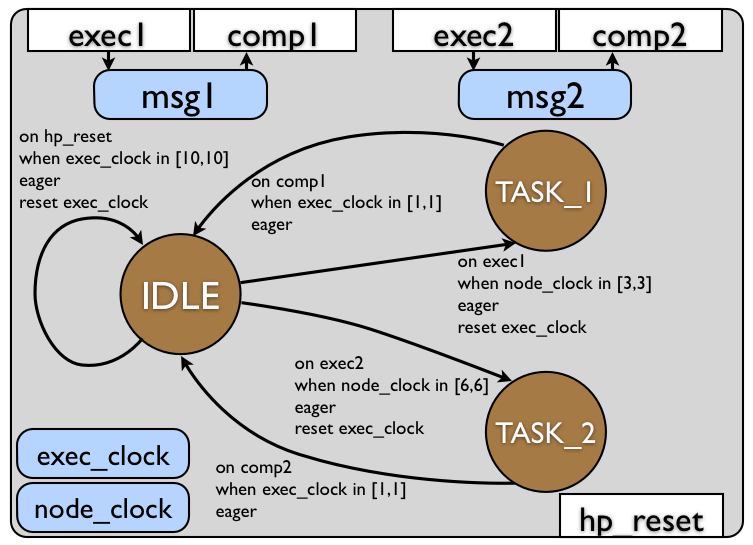
\includegraphics[width=0.75\textwidth]{img/task_model.png}
\caption{BIP model of tasks interacting indirectly by exchanging timed messages on the bus.}
\label{fig:task_model}
\end{figure}


\emph{ESMoL High-Confidence Design Tools}

The Embedded 
Systems Modeling Language (ESMoL) is a suite of 
domain-specific modeling languages (DSML) to integrate the 
disparate aspects of a safety-critical embedded systems design 
and maintain proper separation of concerns between control 
engineering, hardware specification, and software development 
teams\cite{jp_esmol}.  The Embedded Systems Modeling Language (ESMoL) encodes 
in models the relationships between controller functions
specified in Simulink, software components that implement
those functions (i.e. dataflow, messaging interfaces, 
etc\ldots), and the hardware platform on which the software
will run. The language and its associated tools provide the following capabilities:


\begin{itemize}

\item Provide a unified embedded software design environment 
so that modeling, analysis, 
simulation, and code generation artifacts are all 
clearly related to a single design model. ESMoL models use language-specified relations to associate Simulink 
control design structures with
software and hardware design concepts to define a
software implementation for controllers.

\item Include objects and parameters 
to describe deployment of software components to 
hardware platforms.  Analysis artifacts and simulation 
models generated from ESMoL models contain 
representations of the behavioral effects of the 
platform on the original design.

\item Integrate scheduling analysis
so that static schedules can be calculated in rapid design and
simulation cycles.  We include automatic generation of platform-specific
task configuration and data communications code in order to
rapidly move from modeling and analysis to testing on actual hardware.

\item Generate analysis models and code 
using simple template generation techniques.
Round-trip incorporation of calculated schedule 
analysis results back into the ESMoL model helps to
maintain consistency as models pass between design phases.

\end{itemize}

\begin{figure}[thpb]
\centering
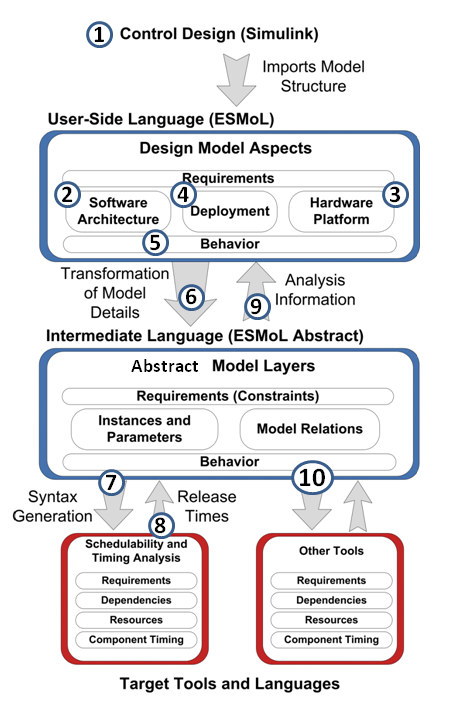
\includegraphics[width=0.75\textwidth]{img/designflow.png}
\caption{Design flow supported by the ESMoL tools.}
\label{fig:designflow}
\end{figure}

Fig. \ref{fig:designflow} illustrates the steps of the ESMoL design flow process\cite{jp_esmol}:

\begin{enumerate}
\item Import a Simulink controller design into an ESMoL model.
\item Specify software component functions and interfaces, and instantiate the components into a logical software architecture model.  At this point functional code generation can take place.
\item Specify the hardware topology for a time-triggered distributed processing network.
\item Define the logical dataflow between software component instances, and the deployment of the logical dataflow to the hardware.
\item Give timing parameters for the tasks and messages in the system.
\item Transform the ESMoL model into a flattened model (ESMoL\_Abstract), resolving all implied model relationships.
\item Transform the ESMoL\_Abstract model into analysis models (such as scheduling problem specifications). Run the analysis.
\item Import results from the analysis back into the ESMoL\_Abstract for consumption by other tools.
\item Import results from the analysis in the ESMoL model (for the user).
\item Generate platform-specific simulations and deployable code from ESMoL\_Abstract.
\end{enumerate}

The control design models provide task period configurations, and 
either profiling or static analysis provides worst-case 
execution time parameters for each component instance.  
Data transfer rates and overhead parameters for communication
buses are stored in the platform model. \cite{jp_tt_sched}
describes the mapping of model structure, execution information,
and platform parameters into actual constraint model details. The Gecode constraint programming
tool solves these constraints for task release and
message transfer times on the time-triggered platform. The scheduling process
should guarantee that the implementation meets the timing requirements 
required by the control design process.

\begin{table*}
\centering
\begin{alltt}
Resolution 1ms

Proc RS 4MHz 0s 0s
Comp InnerLoop =50Hz 1.9ms
Comp DataHandling =50Hz 1.8ms
Comp SerialIn =50Hz 1us
Comp SerialOut =50Hz 1ms
Msg DataHandling.sensor_data_in 1B RS/SerialIn RS/DataHandling 
Msg InnerLoop.thrust_commands 37B RS/InnerLoop RS/SerialOut
Msg DataHandling.ang_msg 1B RS/DataHandling RS/InnerLoop 

Proc GS 100MHz 0s 0s
Comp RefHandling =50Hz 1us
Comp OuterLoop =50Hz 245us
Msg RefHandling.pos_ref_out 9B GS/RefHandling GS/OuterLoop 

Bus TT_I2C 100kb 1.3ms
Msg OuterLoop.ang_ref 20B GS/OuterLoop RS/InnerLoop 
Msg DataHandling.pos_msg 8B RS/DataHandling GS/OuterLoop 
\end{alltt}
\caption{Scheduling spec for the Quadrotor example.}
\label{code:qr_spec}
\end{table*}

\begin{table*}
\centering
\begin{alltt}
\scriptsize
Resolution \{\{RESOLUTION\}\}

\{\{\#HOST_SECTION\}\}Proc \{\{NODENAME\}\} \{\{NODEFREQ\}\} \{\{SENDOHD\}\} \{\{RECVOHD\}\}
\{\{\#TASK_SECTION\}\}Comp \{\{TASKNAME\}\} =\{\{FREQUENCY\}\} \{\{WCEXECTIME\}\}
\{\{\/TASK_SECTION\}\}\{\{\#LOCAL_MSG_SECTION\}\}Msg \{\{MSGNAME\}\} \{\{MSGSIZE\}\} \{\{SENDTASK\}\} \{\{RECVTASKS\}\}
\{\{\/LOCAL_MSG_SECTION\}\}
\{\{\/HOST_SECTION\}\}
\{\{\#BUS_SECTION\}\}Bus \{\{BUSNAME\}\} \{\{BUSRATE\}\} \{\{SETUPTIME\}\} \{\{\#BUS_HOST_SECTION\}\}\{\{NODENAME\}\} \{\{\/BUS_HOST_SECTION\}\}
\{\{\#MSG_SECTION\}\}Msg \{\{MSGNAME\}\} \{\{MSGSIZE\}\} \{\{SENDTASK\}\} \{\{RECVTASKS\}\}
\{\{\/MSG_SECTION\}\}
\{\{\/BUS_SECTION\}\}
\{\{\#LATENCY_SECTION\}\}Latency \{\{LATENCY\}\} \{\{SENDTASK\}\} \{\{RECVTASK\}\}
\{\{\/LATENCY_SECTION\}\}
\end{alltt}
\caption{Stage 2 Interpreter Template for the Scheduling Specification}
\label{code:sched_templ}
\end{table*}

Scheduling specifications are created in the Stage 2 interpreter from
the template shown in Table \ref{code:sched_templ}.
The Stage 2 scheduler generation logic traverses the 
ESMoL\_Abstract model and fills in the structures
which are used to fill in the template when the 
CTemplate generator is invoked.  
In CTemplate, each \verb${{#...}} {{/...}}$ tag pair delimits a 
section which can be repeated by filling in the proper data 
structure in the code.  The other tags \verb${{...}}$ are 
replaced by the string specified in the generation code. 

Producing the \emph{Proc} and \emph{Comp} lines from the model 
API is straightforward as the output mirrors the model
hierarchy, so these lines require only simple traversals 
of the model.  Each generated line uses parameters 
from the respective model object to fill in the blanks.  

In the consraint problem, our scheduler makes use of a global serialization constraint to represent non-preemption\cite{jp_tt_sched}.  The global serialization constraint forces all variable assignments from the given set to be distinct, and to differ by at least a constant value (duration).  For efficiency (and model conciseness), global distinctness constraints are used instead of $n^2$ constraints representing all possibilities.  The scheduler performed well on
randomized problem sets with respect to both execution time and memory usage.

\begin{figure}[thpb]
		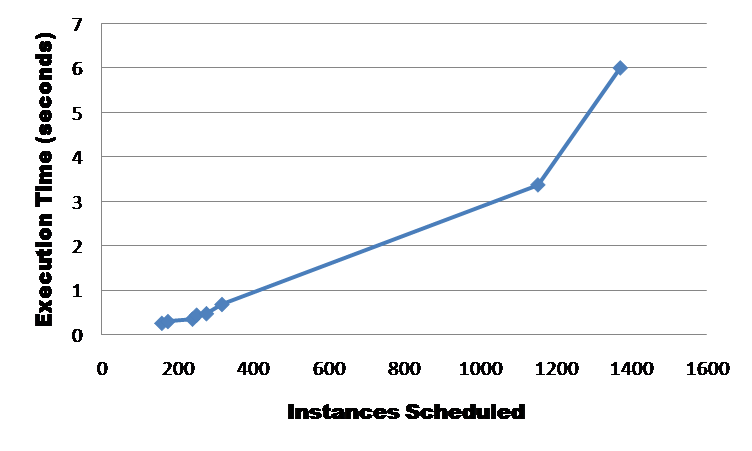
\includegraphics[scale=.7]{img/exectime.png}
		\centering
		\caption{Execution time for feasible instances.}
	  \label{fig:exectime}
\end{figure}

\begin{figure}[thpb]
		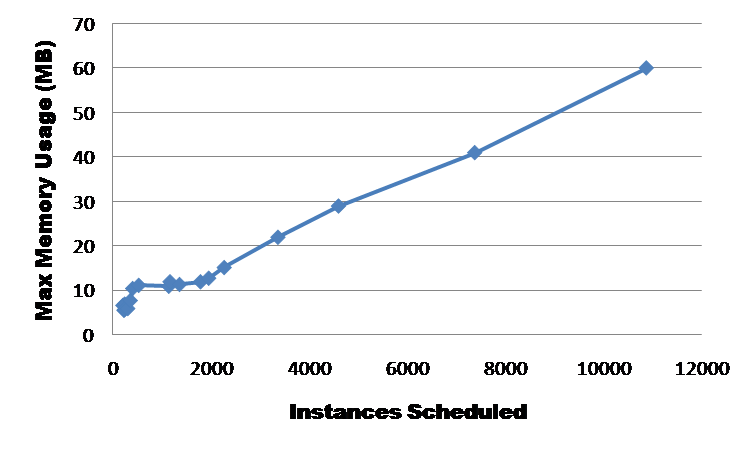
\includegraphics[scale=.7]{img/memusage.png}
		\centering
		\caption{Maximum memory consumption vs. problem instance size.}
		\label{fig:memusage}
\end{figure}

\emph{FRODO Portable Time-Triggered Runtime}

The experimental platform includes a Linux-based TTA realization (the FRODO TTA virtual
machine, running on a low-end ARM Linux board, called the Gumstix platform) and an RTOS-based
TTA realization (the same virtual machine, running on a low-end AVR board, called
the Robostix platform). The same hardware platforms are used in one version of the STARMAC quadrotor.
We have developed platform-specific code generators that create task and communication wrappers for functional
code which will run on the FRODO VM.  We also create I/O drivers for the low-end controller that work with the
time-triggered run-time scheduler and can be targeted by the generators. 

Our tools also implement the FRODO TTA virtual machine logic and timing directly on the TrueTime kernel using the C++ API, to ensure that the platform-included TrueTime model has the same execution semantics as the FRODO runtime on the target hardware\cite{gh_truetime}. 
The TrueTime interface makes the high-fidelity simulation based analysis of controller designs feasible. The actual functional code and the actual schedule are used in the analysis; hence the platform effects are directly observable.  Observations on this simulation provide valuable feedback for the designer on how well the actual controller implementation will work in the real environment. Once the design is found satisfactory, the code can be generated and deployed on the actual controller platform and its performance studied using a hardware-in-the-loop simulation.
Validation of the TrueTime models for the quadrotor uncovered the existence of extra time delay states in the target hardware implementation due to double-buffering on the sensor data receiver.  The TrueTime model was updated to account for the buffer delay.


\begin{figure}[thpb]
\centering
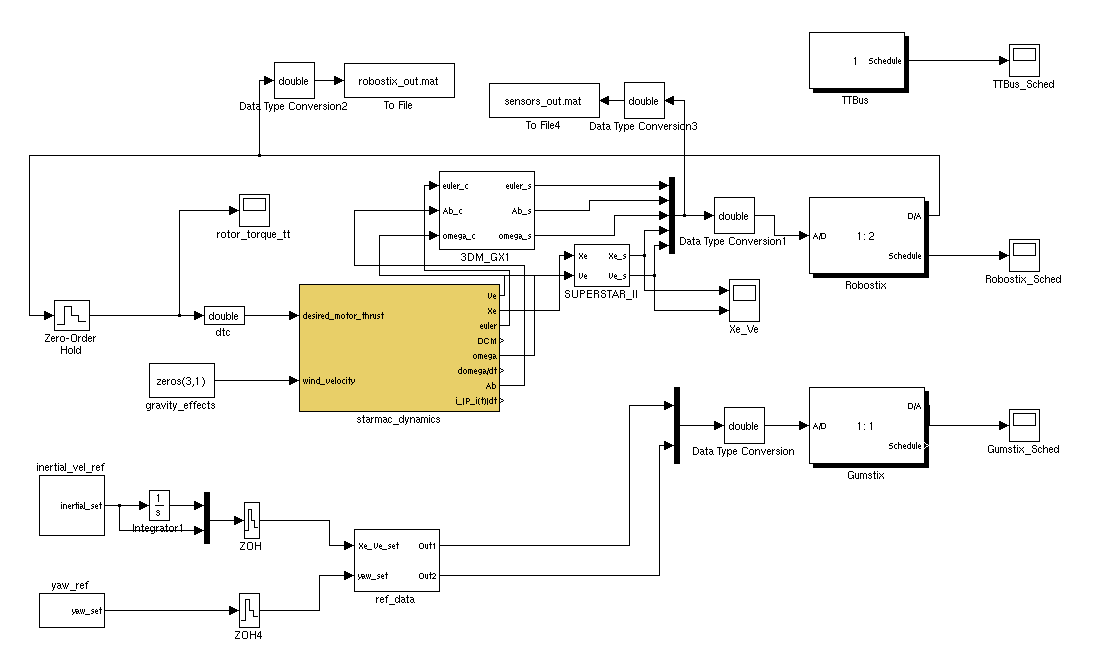
\includegraphics[width=0.9\textwidth]{img/qr_tt}
\caption{TrueTime model of the Starmac quadrotor, including the processor execution timing effects and data networking.}
\label{fig:qr_tt}
\end{figure}



\emph{Other Relevant Tools and Techniques for Design Evaluation}

We have a prototype integration of the CMU statistical model checking tools with our STARMAC model to analyze the robustness of our design to fault conditions.  We give a simple example to illustrate the use of statistical model checking in the quadrotor model.  Fig. \ref{fig:fault1} depicts a fault scenario where the height sensor data includes intermittent (and frequent) glitches which are orders of magnitude larger than the valid data samples (center of the figure).  The traces of the simulated velocity trajectory (right) show that the change in quadrotor height over time has become noisy.  The noise is further aggravated by time delays introduced in the distributed implementation of the controller (lower right).  We would like to formally pose the question of whether the faulty sensor has destabilized the controller and/or its implementation. 

\begin{figure}[thpb]
\centering
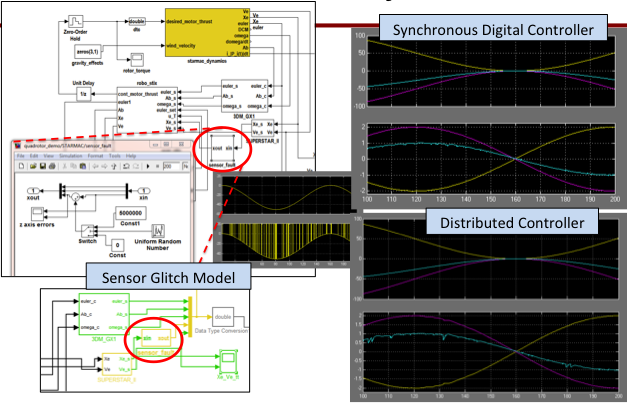
\includegraphics[width=0.9\textwidth]{img/FaultModeling}
\caption{Injection of an aggravated sensor spike fault into the quadrotor behavior. We need to see whether this fault
 causes instability in the distributed deployment of the controller software.}
\label{fig:fault1}
\end{figure}

Fig. \ref{fig:fault2} shows the model framework in Simulink for the use of the Bayesian statistical model checking
\cite{PZ_smc} to evaluate the stability of the control loop with the fault included. The MFOTL block implements 
the interface of the model checker with the Simulink runtime.  The model checking block is configured with an LTL 
condition ``F[0,100s] f1 > 250''.  This sets a hard threshold within which the quadrotor's height must remain during the time specified (100 seconds). A script (bottom of Fig. \ref{fig:fault2}) repeatedly runs the simulation and collects statistics on whether the simulated quadrotor with faulty behavior has destabilized the system. 
In statistical model checking, scalability is still a major issue. We were able to achieve 90\% confidence for this test case in 19 minutes on a 2 GHz processor, but 99\% confidence required 156 minutes.

\begin{figure}[thpb]
\centering
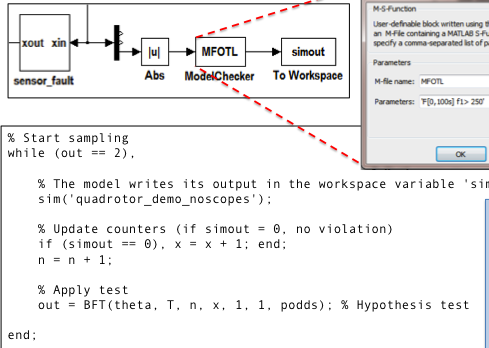
\includegraphics[width=0.9\textwidth]{img/FaultModeling2}
\caption{Addition of the integrated model-checking block, together with the safety condition and execution script.}
\label{fig:fault2}
\end{figure}

We have created prototype extensions to the ESMoL language to support design flows (Fig. \ref{fig:fault3}) which capture the details of fault scenarios and test cases which evaluate those scenarios (Fig. \ref{fig:fault4}).  The intent is to model faulty behavior separately from the nominal design, and to generate statistical model checking simulations as needed which include fault behaviors, conditions, and inputs.

\begin{figure}[thpb]
\centering
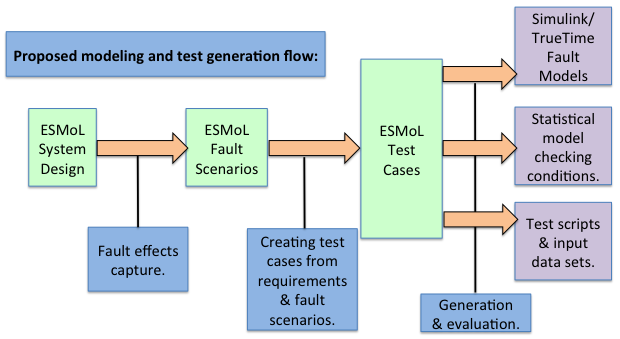
\includegraphics[width=0.9\textwidth]{img/FaultModeling3}
\caption{Proposed design flow to be supported by ESMoL language extensions for fault modeling and testing.}
\label{fig:fault3}
\end{figure}


\begin{figure}[thpb]
\centering
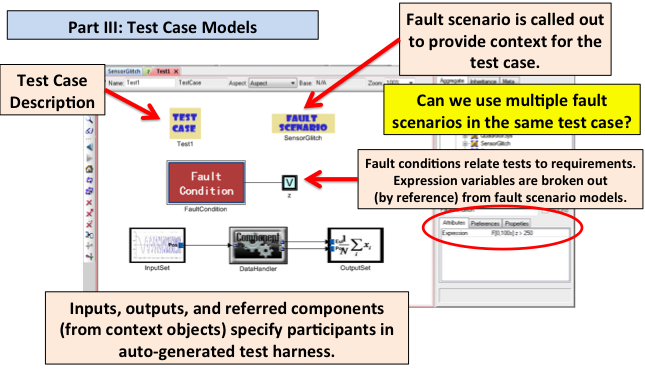
\includegraphics[width=0.9\textwidth]{img/FaultModeling4}
\caption{Test bench language prototype for ESMoL. This concept has been successfully implemented in the CyPhyML system design language and tools (DARPA AVM META project).}
\label{fig:fault4}
\end{figure}



\emph{Pluggable Interpreter Development Architecture}

Fig. \ref{fig:designflow} depicts a design flow 
that includes a user-facing modeling language 
for design and an abstract intermediate language 
for supporting interpreter development and
maintenance.  In our tools, a completed ESMoL model is 
transformed via the Stage 1 
transformation into a model in the ESMoL\_Abstract 
language, where all implied relationships and structural 
model inferences have been resolved (Fig. \ref{fig:stage1}).  
The first model transformation 
flattens the user model into the abstract intermediate form,
translating parameters and resolving special cases as needed. 
Model interpreters 
for calculating time-triggered schedules, creating 
platform-specific simulations, and generating deployable 
code are integrated using the Stage 2 transformation (Fig. \ref{fig:stage2}).
Because generators for code and analysis are attached to the abstract 
modeling layer, so the simpler second-stage transformations 
are easier to maintain, and are isolated from changes to 
the user language and tools.

\begin{figure}[thpb]
\centering
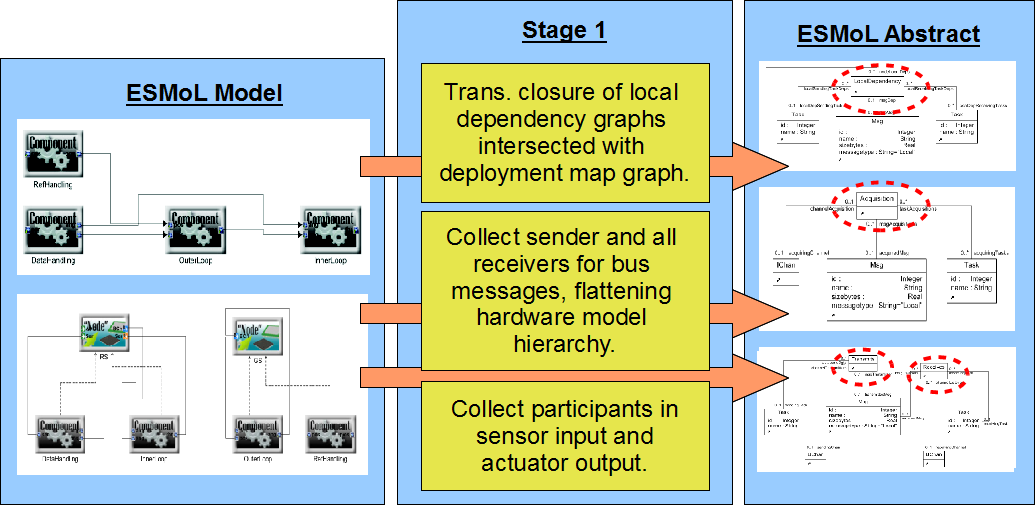
\includegraphics[width=0.9\textwidth]{img/stage1}
\caption{Stage 1 of the ESMoL interpreter framework, which resolves structural inferences and creates a flattened deployment model.}
\label{fig:stage1}
\end{figure}

\begin{figure}[thpb]
\centering
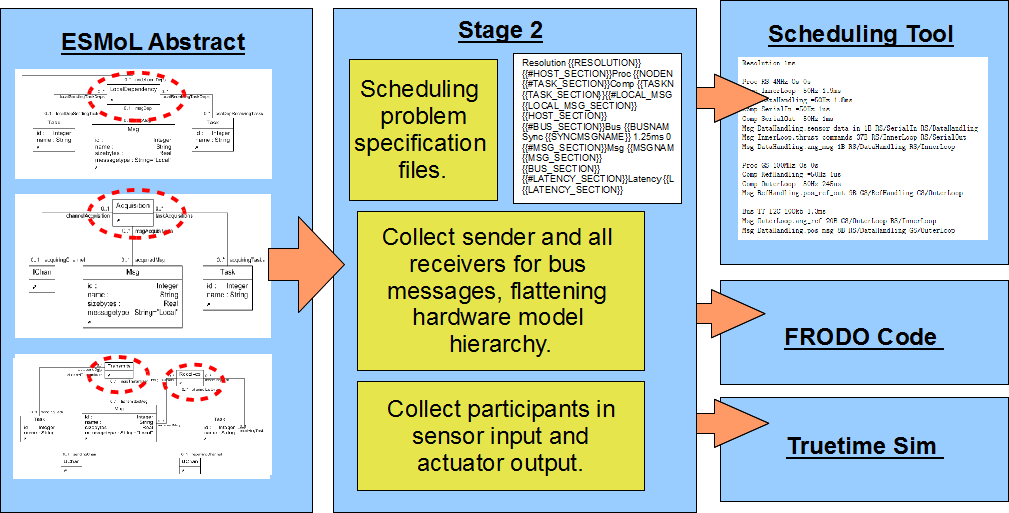
\includegraphics[width=0.9\textwidth]{img/stage2}
\caption{Stage 2 of the ESMoL interpreter framework, which performs the actual transformations. A SystemC target is currently under development for detailed hardware design and evaluation.} 
\label{fig:stage2}
\end{figure}

In the model integrated computing approach, domain specific 
modeling languages represent different aspects of the design, 
with the aim  of consistently integrating different concepts 
and details for those design aspects and integrated analysis tools.
This architecture makes interpreter development simpler, extending the language composition
capabilities of the MIC tools with greater composability for modeling language tools as well.
Fig. \ref{fig:sched_integration} depicts the details of one example of such a
transformation, the schedule problem generation described previously.

\begin{figure}[thpb]
\centering
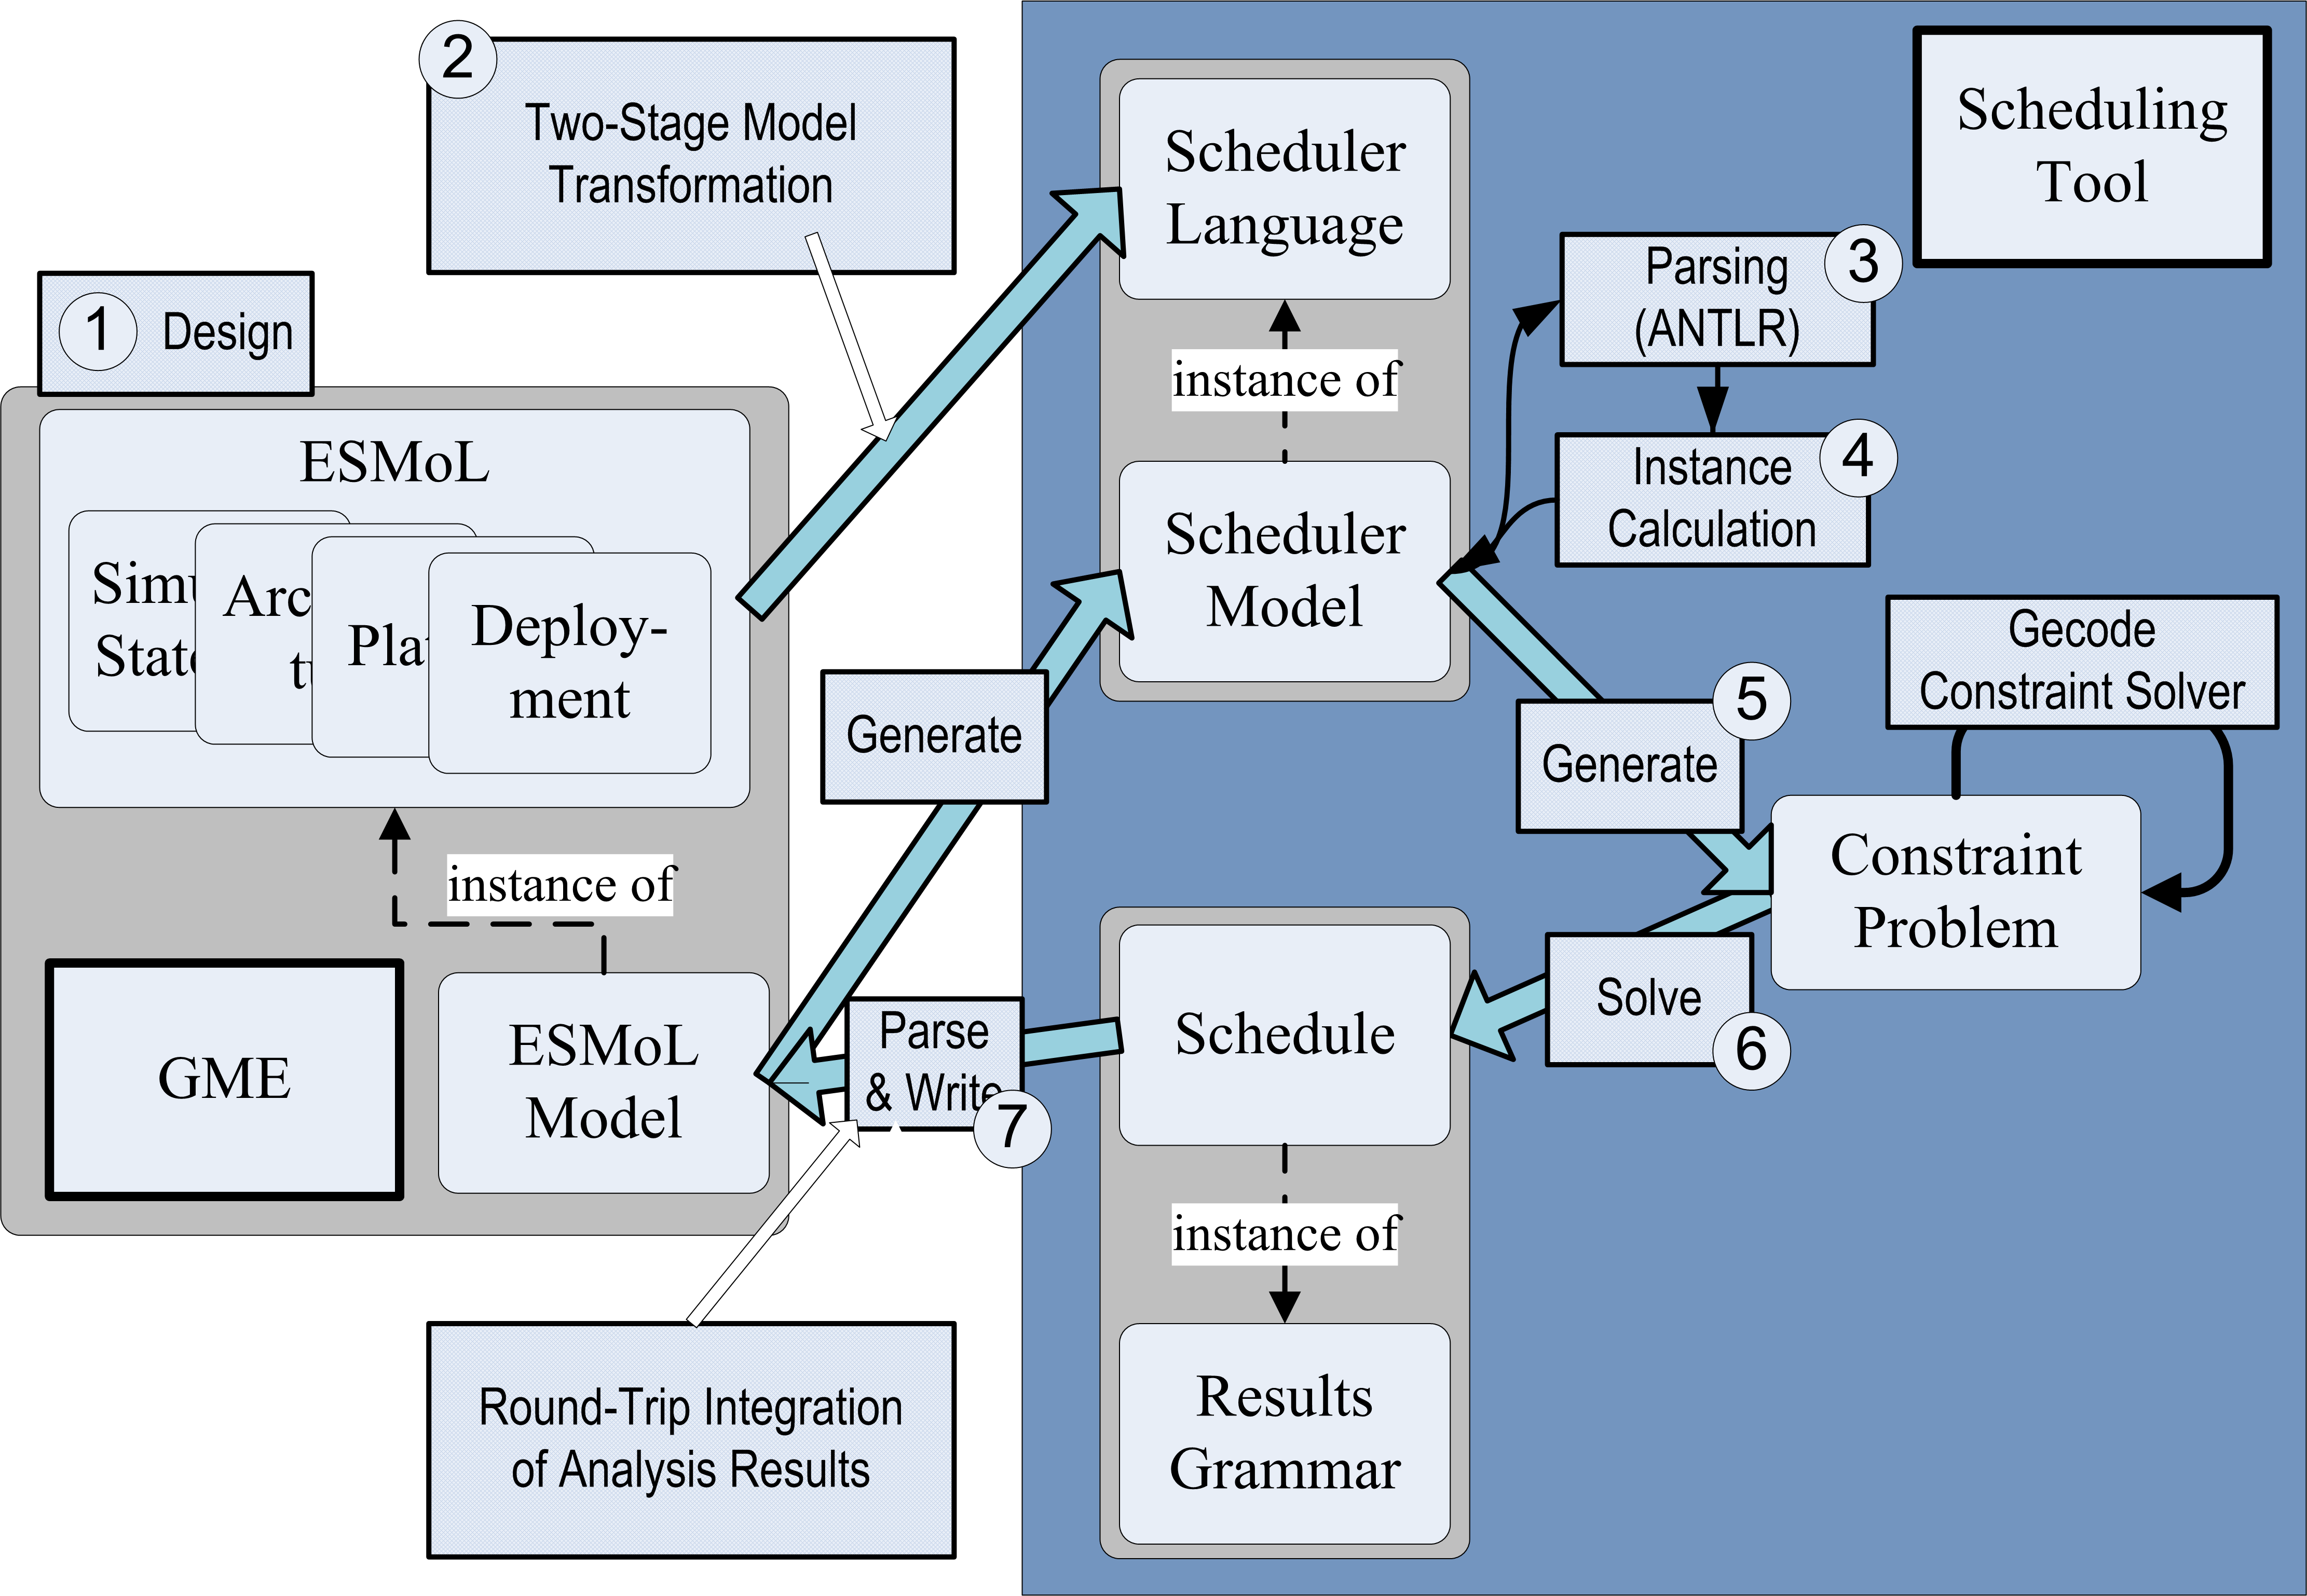
\includegraphics[width=0.9\textwidth]{img/sched_integration}
\caption{Example: Stage 2 generates scheduling problem specifications using the Stage 1 results and output templates. Results are parsed and written back into the source model.} 
\label{fig:sched_integration}
\end{figure}


\subsubsection{Controlling Timing with a deadline instruction (Lee)}

	      
	      We have enabled control over timing at the ISA level by
               introducing four so-called ``deadline''
               instructions. As higher-level models of computation
               (MoC) often have a timed semantics, the deadline
               instructions can be used to implement such MoCs at the
               binary level, thereby filling a void in the model-based
               development of high-confidence systems from high-level
               models to low-level realizations. To allow for a wide
               range of cost-efficient implementations of the PRET
               timed semantics, it can be parameterized in different
               architectural aspects, as for instance the sizes of
               different levels of the memory hierarchy. We have made
               significant progress in developing parametric timing
               analyses to support the verification of timing
               constraints on PRET.

               On the implementation side, we have continued the
               development of a prototypical PRET processor called
               PTARM, implementing the four deadline instructions and
               providing predictable timing behavior. A new PRET DRAM
               controller provides access to large Dynamic RAMs at
               predictable and composable memory access times to the
               four hardware threads of the PTARM core. Compared with
               previous approaches, we improve the worst-case access
               latency of small requests by up to 73\%.
               
               Report:
               
               Guaranteeing the correct behavior of embedded systems
               is extremely difficult, especially with respect to
               timing constraints and their relationship to the safety
               of the physical systems. The traditional verification
               process is faced with two major challenges regarding
               timing constraints: 1. The execution time of a program
               depends on the hardware on which it is running. Every
               new hardware realization requires the development of
               new timing analysis tools. 2. The development process
               of such analysis tools is becoming increasingly
               error-prone and time-consuming for modern, complex
               hardware realizations.

               PRET tackles both of these challenges. By introducing a
               timed semantics for the instruction set architecture,
               timing becomes a property of programs rather than a
               property of programs running on particular hardware
               realizations. As a consequence, programs can be ported
               from one realization to the next without having to
               recertify and develop new timing analysis
               tools. Furthermore, due to the simplicity of the timing
               model associated with the ISA, precise and efficient
               timing analysis becomes possible. We anticipate this
               work to entail a paradigm shift in the development of
               hardware realizations for embedded systems: instead of
               focusing on improving performance, new hardware
               realizations will be developed that optimize aspects
               such as energy and power consumption, implementation
               cost, and reliability.

               In the past year, we have taken the following steps towards the PRET vision: 
               \begin{itemize}

               \item We have introduced four so-called ``deadline''
                 instructions, which introduce control over timing
                 at the ISA level. These instructions allow to
                 enforce upper and lower bounds on the execution
                 time of blocks of code and provide the ability to
                 act upon deadline misses. As higher-level models of
                 computation (MoC) often have a timed semantics, the
                 deadline instructions can be used to implement such
                 MoCs at the binary level, thereby filling a void in
                 the model-based development of high-confidence
                 systems from high-level models to low-level
                 realizations. This work
                 \cite{Reineke11_PRETDRAMControllerBankPrivatizationForPredictability}
                 has been presented at DAC 2011.

               \item We have continued the development of a
                 prototypical PRET processor called PTARM, which
                 shall implement the four deadline instructions and
                 provide predictable timing behavior \cite{LiuReinekeLee10_PRETArchitectureSupportingConcurrentProgramsWithComposable}.

               \item We have developed a new DRAM controller which
                 provides predictable and composable memory access
                 times to the four hardware threads of the PTARM
                 core. Instead of viewing the DRAM device as one
                 resource that can only be shared as a whole, our
                 approach views it as multiple resources that can be
                 shared between one or more clients individually. We
                 partition the physical address space following the
                 internal structure of the DRAM device, i.e., its
                 ranks and banks, and interleave accesses to the
                 blocks of this partition. This eliminates
                 contention for shared resources within the device,
                 making accesses temporally predictable and
                 temporally isolated. Compared with previous
                 approaches, we improve the worst-case access
                 latency of small requests by up to 73\%. This work
                 \cite{Reineke11_PRETDRAMControllerBankPrivatizationForPredictability},
                 has been presented at CODES+ISSS 2011.

               \item To allow for a wide range of cost-efficient
                 implementations of the PRET timed semantics, it can
                 be parameterized in different architectural
                 aspects, as for instance the sizes of different
                 levels of the memory hierarchy and their respective
                 latencies, or the latencies floating-point
                 instructions. Supporting such a parameterized timed
                 semantics requires parametric timing
                 analysis. Parametric timing analysis derives a
                 predicate that is satisfied for choices of
                 parameter values that are guaranteed to meet all
                 timing constraints. This summer, we have made
                 significant progress in developing such parametric
                 analyses.

               \end{itemize}


